\vspace{-.1cm}
\section{Introduction}
\vspace{-.1cm}
\begin{figure}[t!]
  \centering
  \vspace{-2em}
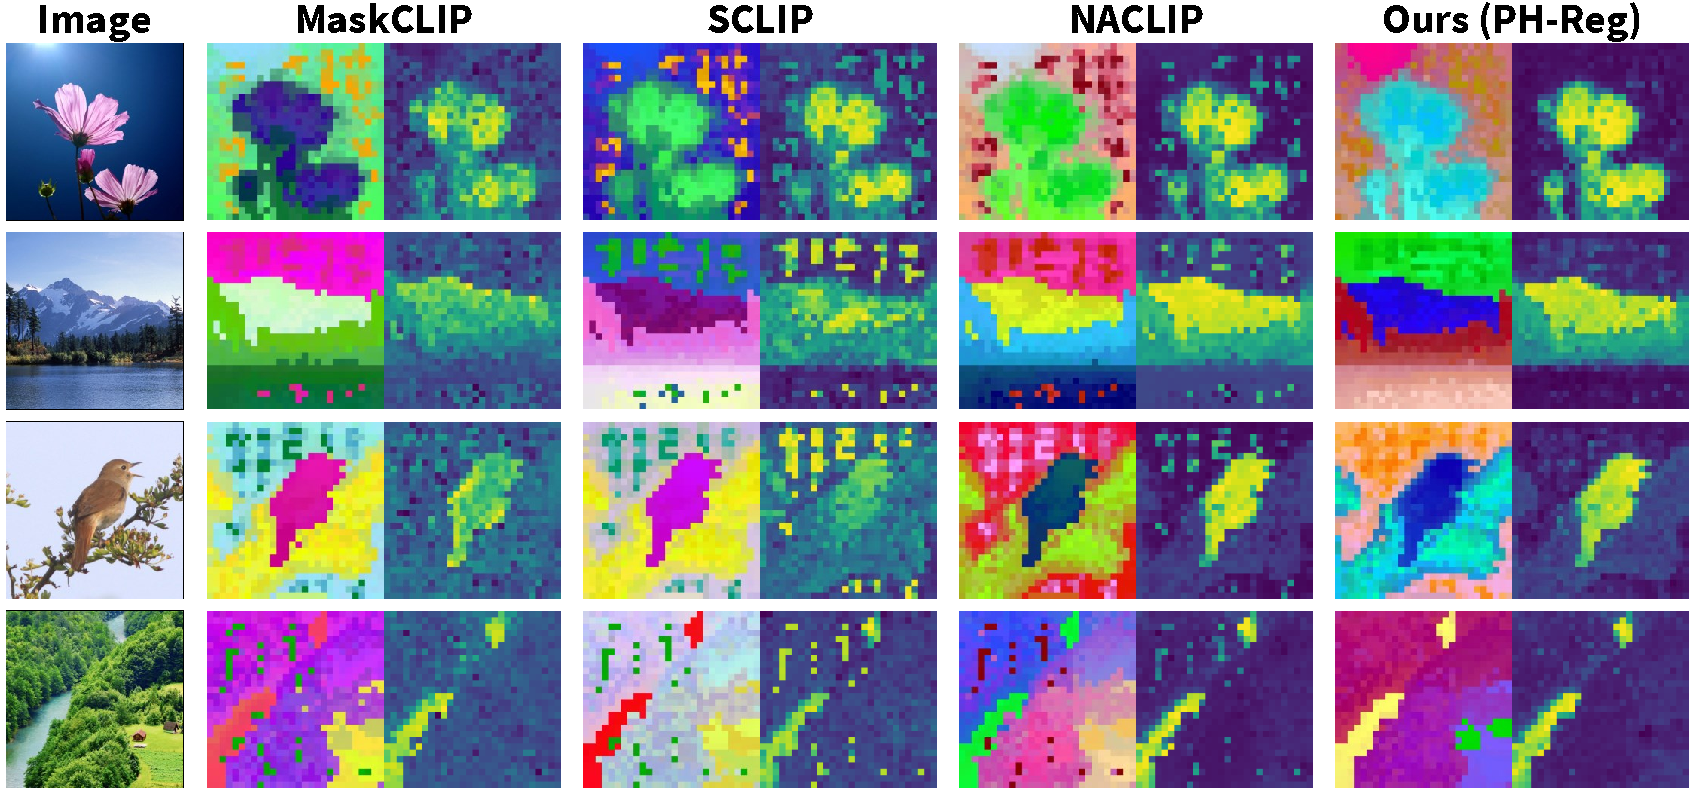
\includegraphics[width=0.95\linewidth]{fig_pdf/teaser.pdf}
  \caption{\textbf{Effect of PH-Reg on Open-vocabulary Segmentation.} For each image, we compare four methods: MaskCLIP which directly takes the \emph{value} features from the last attention layer; SCLIP which adds correlative self-attention; NACLIP which further enforces a locality bias; and our PH-Reg method with self-distilled registers. We utilize the same \texttt{OpenAI CLIP ViT-B/16} weights for all three methods. For each method, we visualize the UMAP of the dense features and a heatmap of one text query. Our method yields noticeably cleaner dense features and high quality localizations, and requires only a small set of additional register parameters compared to the original network.}
  \vspace{-0.2cm}
  \label{fig:teaser}
\end{figure}
Vision Transformers (ViTs) are now the dominant architecture in visual modeling, delivering strong performance across classification, detection, and segmentation. Unlike convolutional networks with their built-in locality inductive bias, ViTs process images by spatially splitting them into patches and applying self-attention to enable global feature interactions. This architectural design leads to superior scalability, particularly with contrastive or self-supervised pre-training objectives, and facilitates more flexible representation learning, as it is less constrained by the translation invariance assumptions inherent in CNNs. This flexibility enables remarkable emergent capabilities. Models like CLIP, trained solely on image-text alignment, achieve competitive open-vocabulary segmentation through zero-shot dense queries; while self-supervised approaches learn semantically rich features directly from unlabeled images. 

However, the same data-driven attention mechanisms that enable ViT's representation power can also lead to the emergence of \emph{artifact tokens}. These are outlier features often discordant with local image semantics, meaning they fail to correspond to locally meaningful image structures. The propensity for ViTs to generate such tokens is exacerbated by their lack of strong, built-in spatial priors, which can result in inconsistent dense representations. Ultimately, the presence of these artifact tokens disrupts fine-grained localization, a critical capability for tasks demanding high spatial precision, such as detailed semantic segmentation or part identification.

Recent work has sought to mitigate artifact tokens via architectural modifications, where \textit{register tokens} are added to the network. These register tokens are randomly initialized, with learnable parameters that participate in the self-attention process similar to the \texttt{[CLS]} token, but are not otherwise used during the output. Although these register tokens are not explicitly supervised during training, they effectively ``absorb'' the artifact term and learn to attend to global objects. While effective, introducing register tokens constitutes a fundamental architectural modification that requires training from scratch---a time-consuming and computationally demanding process. This significantly limits their applicability, especially given the vast ecosystem of \emph{existing, high-performing pre-trained vision models.} 

We present a solution to this issue with \textbf{P}ost \textbf{H}oc \textbf{Reg}isters (\textbf{PH-Reg}), an efficient self-distillation framework that requires no labeled data or full retraining. We illustrate OpenAI CLIP with PH-Reg in Figure~\ref{fig:teaser}. In PH-Reg, both teacher and student networks are initialized from the same pre-trained model weights. And the only extra parameters are the register tokens added to the student network. Our proposed framework freezes the teacher during training. Images provided to the teacher undergo test-time augmentation (e.g. random offsets and horizontal flips). This augmentation strategy effectively denoises the teacher's dense features without requiring gradient-based updates on the teacher itself, yielding stable dense targets. The denoised dense features are used as a distillation target for the student network, where only a small set of parameters are optimized. This entire process requires only a modest set of unlabeled images, enabling significant enhancements to pre-trained models with minimal computational overhead. Concretely our contributions are as follows: \textbf{1.} We propose a test-time augmentation scheme that can effectively denoise dense features in vision transformers. Our denoiser does not require costly neural fields and does not require gradient based optimization. \textbf{2.} We elucidate the underlying components in a student model that contribute to learning a clean dense feature map. We show that by finetuning select weights, we are able to achieve clean dense features with minimal additional parameters. \textbf{3.} We demonstrate that PH-Reg effectively improves the consistency of dense feature representations in ViTs, leading to quantifiable improvements on downstream tasks that rely on fine-grained spatial understanding (e.g., semantic segmentation or depth prediction). Our method preserves the original utility of dense features without inducing unwanted distribution shift, and functions well with zero-shot language-based dense queries. 
